\paragraph{A raw target moment repairs an avoidable compression loss.}
A reaction-only diagnostic starts from one with rate $20(1+0.95\sin(2\pi x))$ and final time one. It creates unresolved structure on a coarse FE mesh. The measured quantity is the error of the FE observation against $P_V\exp(-r)$, not the continuous-field approximation error. The exact coarse Galerkin matrix exponential provides a separate closure comparator.
\begin{center}\small\begin{tabular}{lrr}\toprule Method & Observation error & Evolution (s)\\\midrule
Old three-direction space & 3.294e-03 & 0.2411\\
FE reconstruction & 3.493e-01 & 0.0218\\
Direct auxiliary evolution & 1.286e-10 & 0.0186\\
Raw target, two directions & 2.831e-11 & 0.2232\\
\bottomrule\end{tabular}\end{center}
These are single evolution measurements for $P_1$, $n_V=4$, $Q_4$, $n_W=128$ and 64 steps, excluding preparation. The direct auxiliary solver remains faster and requires no compression in this reaction-only example. Thus the experiment motivates the retained direction but establishes no overall efficiency advantage.
\begin{figure}[htbp]\centering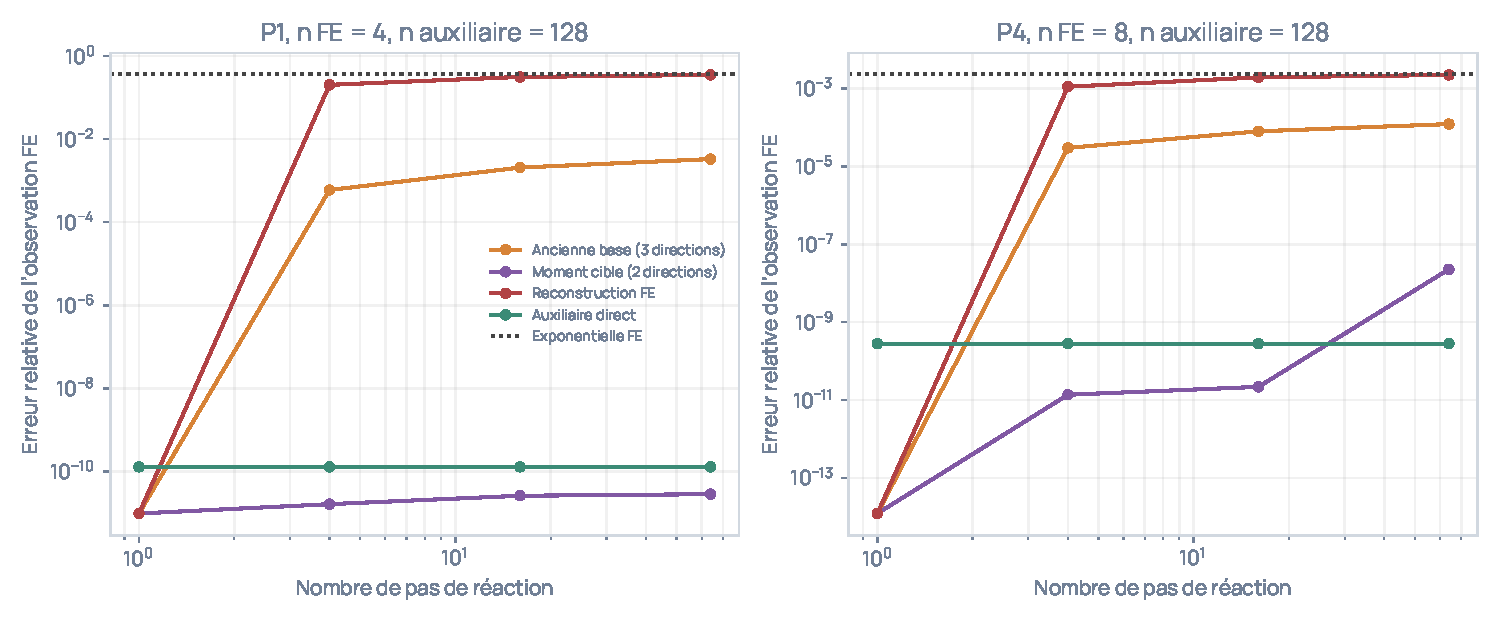
\includegraphics[width=\linewidth]{night-target-seed.pdf}
\caption{Coarse FE observation of an unresolved reaction. Retaining the raw auxiliary target moment substantially reduces compression error. The numerical rank cutoff remains relevant near dependent directions.}\end{figure}
